\section{Correlation matrix} %4.1

\begin{figure}[htbp]
\centering
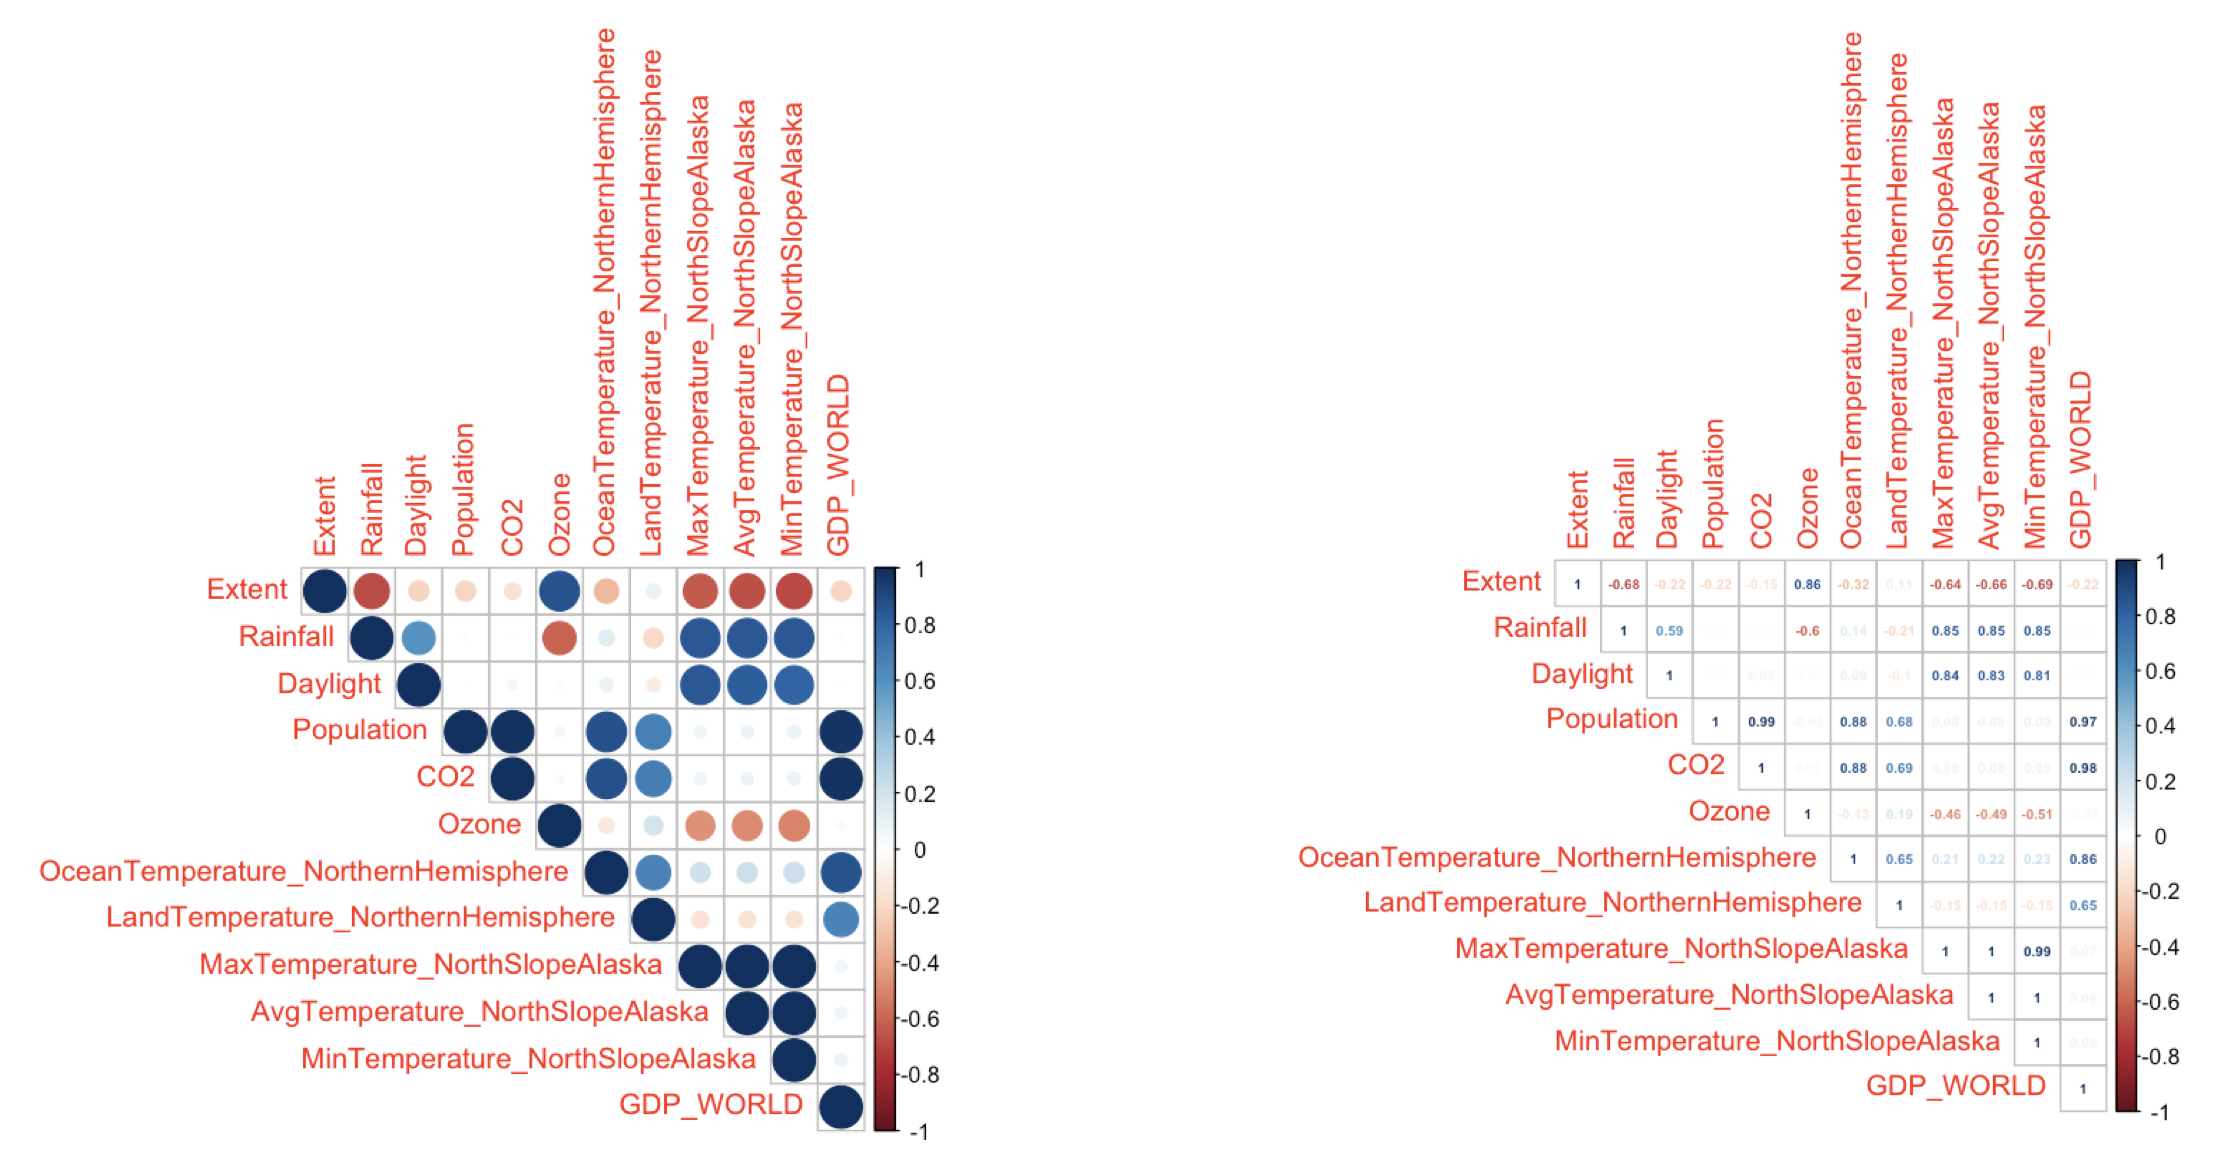
\includegraphics[width = 1.0\textwidth]{Figure/4.1-CM.png}
\caption{Left: The correlation matrix with "circle" method. Right: The correlation matrix with "number" method.}
\label{4.1-CM}
\end{figure}
The correlation matrix is a symmetric matrix. Based on the results of the Correlation Matrix, it shows that the extent of Arctic sea ice has a strong correlation with ozone, temperature gained from North Slope Alaska, and rainfall. The temperature measured in the North Pole Alaska is divided into maximum, average, and minimum temperatures. These three measured temperature values are not only highly correlated with extent but also highly correlated with each other. Therefore, it is unreasonable to add all three variables into the model. Here, the feature with the greatest correlation (min temperature) was selected by Correlation Matrix through number but not through symbol. Hence, the minimum temperature gained from North Slope Alaska was selected.